\chapter{Rilassamento Lagrangiano per il calcolo di lower bounds}
Si consideri il seguente problema $P$ di programmazione a numeri interi:
\begin{displaymath}
P:
\begin{cases}
	z(P)=Min\;cx \\
	\;\;\;\;\;\;\;\;\;\;\;\;s.t.\;Ax\ge b \\
	\;\;\;\;\;\;\;\;\;\;\;\;\;\;\;\;\;\;Bx\ge d \\
	\;\;\;\;\;\;\;\;\;\;\;\;\;\;\;\;\;\;x\in\{0,1\}^{n} 
\end{cases}
\end{displaymath}
Il valore ottimo $z(LP)$ del rilassamento lineare $LP$ del problema $P$ fornisce un valido lower bound, ovvero
\begin{equation}
	z(LP)\le z(P)
\end{equation}
$LP$ si ottiene da $P$ sostituendo $x\in\{0,1\}^{n}$ con $0\le x\le 1$:
\begin{displaymath}
LP:
\begin{cases}
z(LP)=Min\;cx \\
\;\;\;\;\;\;\;\;\;\;\;\;\;\;\;s.t.\;Ax\ge b \\
\;\;\;\;\;\;\;\;\;\;\;\;\;\;\;\;\;\;\;\;\;Bx\ge d \\
\;\;\;\;\;\;\;\;\;\;\;\;\;\;\;\;\;\;\;\;\;0\le x\le 1
\end{cases}
\end{displaymath}
In molti casi:
\begin{itemize}
	\item è pribitivo risolvere $LP$: troppe variabili e/o vincoli;
	\item $z(LP)$ è troppo distante da $z(P)$ e quindi non utilizzabile in un algoritmo Branch and Bound.
\end{itemize}

\section{Rilassamento Lagrangiano di $P$ rispetto ai vincoli $Ax\ge b$}
Viene così definito il problema $RL_{u}$ che si ottiene da $P$ rimuovendo i vincoli $Ax\ge b$ e sottraendo dalla funzione obiettivo il termine $u(Ax-b)$ dove $u\ge 0$ è il vettore dei \textbf{Moltiplicatori Lagrangiani}.
\begin{displaymath}
	RL_{u}:
	\begin{cases}
		L(u)=Min\;cx-u(Ax-b) \\
		\;\;\;\;\;\;\;\;\;\;\;\;s.t.\;Bx\ge d \\
		\;\;\;\;\;\;\;\;\;\;\;\;\;\;\;\;\;\;x\in\{0,1\}
	\end{cases}
\end{displaymath}
$L(u)$ viene detta "\textit{Funzione Lagrangiana}"

\subsection{Esempio}
\begin{displaymath}
P:
\begin{cases}
z(P)=Min\;3x_{1}+7x_{2}+10x_{3} \\
\;\;\;\;\;\;\;\;\;\;\;\;s.t.\;x_{1}+3x_{2}+5x_{3}\ge 7 \\
\;\;\;\;\;\;\;\;\;\;\;\;\;\;\;\;\;\;x_{1},x_{2},x_{3}\in\{0,1\}
\end{cases}
\end{displaymath}
\begin{displaymath}
RL_{u}:
\begin{cases}
L(u)=Min\;x_{1}+7x_{2}+10x{3}-u(x_{1}+3x_{2}+5x_{3}-7) \\
\;\;\;\;\;\;\;\;\;\;\;\;s.t.\;x_{1},x_{2},x_{3}\in\{0,1\}
\end{cases}
\end{displaymath}

\section{Validità e importanza di $RL_{u}$}
Possiamo dimostrare che $L(u)\le z(P),\;\forall u\ge0$ e quindi $\underset{u\ge 0}{Max}[L(u)]\le z(P)$.\\
In certe condizioni la soluzione ottima di $RL_{u}$ è anche la soluzione ottima di $P$.

\subsection{Esempio}
\begin{displaymath}
P:
\begin{cases}
z(P)=Min\;2x_{1}+3x_{2}+4x_{3}+5x_{4} \\
\;\;\;\;\;\;\;\;\;\;\;\;s.t.\;x_{1}+x_{3}\ge 1 \\
\;\;\;\;\;\;\;\;\;\;\;\;\;\;\;\;\;\;x_{1}+x_{4}\ge 1 \\
\;\;\;\;\;\;\;\;\;\;\;\;\;\;\;\;\;\;x_{2}+x_{3}+x_{4}\ge 1 \\
\;\;\;\;\;\;\;\;\;\;\;\;\;\;\;\;\;\;\forall i \in \{0,1\},\;i=1,\dots,4 \\
\end{cases}
\end{displaymath}
La soluzione ottima è $x_{1}=x_{2}=1,\;x_{3}=x_{4}=0$ e $z(P)=S$.\\
Il rilassamento lagrangiano dei tre vincoli richiede tre moltiplicatori $u_{1},u_{2},u_{3}$; quindi
\begin{flalign}
	& (RL_{u})\;\;\;\;L(u))=Min\;2x_{1}+3x_{2}+4x_{3}+5x_{4} -u_{1}(x_{1}+x_{3}-1) \\
	& \;\;\;\;\;\;\;\;\;\;\;\;\;\;\;\;\;\;\;\;\;\;\;\;\;\;\;\;\;\;\;\;\;\;\;\;\;\;\;\;\;\;\;\;\;\;\;\;\;\;\;\;\;\;\;\;\;\;\;\;\;\;\;\;\;\;\;\;\;\;\;-u_{2}(x_{1}+x_{4}-1) \\
	& \;\;\;\;\;\;\;\;\;\;\;\;\;\;\;\;\;\;\;\;\;\;\;\;\;\;\;\;\;\;\;\;\;\;\;\;\;\;\;\;\;\;\;\;\;\;\;\;\;\;\;\;\;\;\;\;\;\;\;\;\;\;\;\;\;\;\;\;\;\;\;-u_{3}(x_{2}+x_{3}+x_{4}-1 ) \\
	&\;\;\;\;\;\;\;\;\;\;\;\;\;\;\;\;\;\;\;\;\;s.t.\; x_{i}\in\{0,1\},\;i=1,\dots,4
\end{flalign}
ma anche
\begin{flalign}
	& (RL_{u})\;L(u)=Min\;(2-u_{1}-u_{2})x_{1}+(3-u_{3})x_{2}+(4-u_{1}-u_{3})x_{3}+(5-u_{2}-u_{3})x_{4}+u_{1}+u_{2}+u_{3} \\
	& \;\;\;\;\;\;\;\;\;\;\;\;\;\;\;\;\;\;\;\;\;\;s.t.\;x_{i}\in\{0,1\},\;i=1,\dots,4
\end{flalign}
Dato $u$, la soluzione ottima di $RL_{u}$ e, conseguentemente, il valore di $L(u)$ si ottiene ponendo
\begin{flalign*}
	& x_{i}=0\textnormal{ se il coefficiente di $x_{i}$ è }\ge 0 \\
	& x_{i}=1\textnormal{ se il coefficiente di $x_{i}$ è }< 0 \\
\end{flalign*}
Poniamo $u_{1}=1.5$, $u_{2}=1.6$ e $u_{3})=2.2$
\begin{equation*}
	L(u)=Min\; -1.1x_{1}+0.8x_{2}+0.3x_{3}+1.2x_{4}+1.5+1.6+2.2
\end{equation*}
La soluzione ottima è
\begin{equation*}
	x_{1}=1,\;x_{2}=x_{3}=x_{4}=0
\end{equation*}
quindi
\begin{equation*}
	L(u)=-1.1+1.5+1.6+2.2=5.3-1.1=4.2
\end{equation*}
Ponendo $u_{1}=1$, $u_{2}=1$ e $u_{3}=3$
\begin{equation*}
L(u)=Min\; 0x_{1}+0x_{2}+0x_{3}+x_{4}+1+1+3
\end{equation*}
Una soluzione ottima è
\begin{equation*}
x_{1}=1=x_{2}=x_{3}=x_{4}=0
\end{equation*}
di costo $L(u)=0+0+0+0+1+1+3=5\equiv z(P)$.\\
Si noti che esistono soluzioni ottime alternative tutte di costo $L(u)$=5 che si ottengono ponendo $x_{1}=1$ e/o $x_{2}=1$ e/o $x_{3}=1$ e $x_{4}=0$. Fra tali soluzioni esiste quella ottima! $x_{1}=x_{2}=1$ e $x_{3}=x_{4}=0$

\section{TEOREMA: Dualità Lagrangiana debole}
Il valore ottimo $z(P)$ del problema
\begin{displaymath}
P:
\begin{cases}
z(P)=Min\;\;cx \\
\;\;\;\;\;\;\;\;\;\;\;\;s.t.\;Ax\ge b \\
\;\;\;\;\;\;\;\;\;\;\;\;\;\;\;\;\;\;Bx\ge d \\
\;\;\;\;\;\;\;\;\;\;\;\;\;\;\;\;\;\;x\in \{0,1\} \\
\end{cases}
\end{displaymath}
è maggiore o uguale al valore ottimo $L(u)$ del problema
\begin{displaymath}
RL_{u}:
\begin{cases}
L(u)=Min\;cx-u(Ax-b) \\
\;\;\;\;\;\;\;\;\;\;\;\;s.t.\;Bx\ge d \\
\;\;\;\;\;\;\;\;\;\;\;\;\;\;\;\;\;\;x\in \{0,1\} \\
\;\;\;\;\;\;\;\;\;\;\;\;\;\;\;\;\;\;\forall u\ge 0 \\
\end{cases}
\end{displaymath}
\subsection{Dimostrazione}
Sia $x^{*}$ la soluzione ottima di $P$. Si noti che $x^{*}$ è anche una soluzione ammissibile per $RL_{u}$ per ogni $u\ge 0$, ma non necessariamente l'ottimo di $RL_{u}$ per un dato $u$.\\
Si ha, quindi, che
\begin{equation}
	cx^{*}-u(Ax^{*}-b)\ge L(u)
\end{equation}
ma $u(Ax^{*}-b)\ge 0$ (poichè $u\ge 0$ e $Ax^{*}\ge b$ essendo per ipotesi $x^{*}$ l'ottimo di $P$); quindi
\begin{equation}
	cx^{*}\ge L(u)\textnormal{ ovvero }z(P)\ge L(u)\;\;\;\;\;\;\;\;\;\;\square
\end{equation}

\section{Lagrangiano Duale}
Dal teorema della dualità debole per cui $L(u)\le z(P)$, $\forall u\ge 0$, si ha che l'ottimo $z(D_{L})$ del seguente problema:
\begin{equation}
	D_{L}\;\;\;\;\;\;z(D_{L})=\underset{u\ge 0}{Max}\;[L(u)]
\end{equation}
è un valido lower bound a $z(P)$; ovvero $z(D_{L})\le z(P)$.\\
Il problema $D_{L}$ è detto \textit{Lagrangiano Duale} di $P$.

\section{Duality Gap}
Nel caso in cui $z(D_{L})<z(P)$ allora si dice che esiste un \textbf{duality gap} fra il problema $P$ e il problema $D_{L}$.\\
Supponiamo che l'ottimo di $D_{L}$ si ottenga risolvendo $L(\bar{u})$ per un dato $\bar{u}\ge 0$, ovvero, $z(D_{L})=L(\bar{u})$.\\
Indichiamo con $\bar{x}$ la soluzione ottima di $RL_{\bar{u}}$ ovvero:
\begin{equation}
	z(D_{L})=L(\bar{u})=c\bar{x}-\bar{u}(A\bar{x}-b)
\end{equation}
Si consideri il caso in cui $\bar{x}$ è anche l'ottimo di $P$, ovvero, $z(P)=c\bar{x}$.\\\\
È evidente che $z(D_{L})<z(P)$ se $\bar{u}(A\bar{x}-b)>0$.

\subsection{Esempio}
\begin{displaymath}
P:
\begin{cases}
z(P)=Min\;3_x{1}+7x_{2}+10x_{3} \\
\;\;\;\;\;\;\;\;\;\;\;\;s.t.\;x_{1}+3x_{2}+5x_{3}\ge 7 \\
\end{cases}
\end{displaymath}
\begin{equation*}
	L(u)=Min\;3x_{1}+7x_{2}+10x_{3}-u(x_{1}+3x_{2}+5x_{3}-7)
\end{equation*}
\begin{equation*}
	x_{1},x_{2},x_{3}\in \{0,1\}
\end{equation*}
Per calcolare $z(D_{L})\underset{u\ge 0}{Max}[L(u)]$ calcoliamo $L(u)$, $u\ge 0$
\begin{flalign*}
	& u=0\;\;\;\;\;\;L(0)=0\;\;\;\;\;\;\;\;\;\;\;\;\;\;\;\;\;x=(0,0,0) \\
	& u=1\;\;\;\;\;\;L(1)=7\;\;\;\;\;\;\;\;\;\;\;\;\;\;\;\;\;x=(0,0,0) \\
	& u=2\;\;\;\;\;\;L(2)=14\;\;\;\;\;\;\;\;\;\;\;\;\;\;\;x=(0,0,0)\textnormal{ oppure }x=(0,0,1) \\
	& u=\frac{7}{3}\;\;\;\;\;L(\frac{7}{3})=\frac{44}{3}\;\;\;\;\;\;\;\;\;\;\;\;\;\;x=(0,0,1)\textnormal{ oppure }x=(0,1,1) \\
	& u=3\;\;\;\;\;\;L(3)=14\;\;\;\;\;\;\;\;\;\;\;\;\;\;\;\;x=(0,1,1)\textnormal{ oppure }x=(1,1,1) \\
	& u>3\;\;\;\;\;\;L(u)=-2u+20\;\;\;\;\;x=(1,1,1) \\
\end{flalign*}
Quindi $z(D_{L})=\frac{44}{3}$ mentre $z(P)=17$ e $x^{*}=(0,1,1)$ che corrisponde ad una delle soluzioni di $L(\frac{7}{3})=\frac{44}{3}$ ma esiste un gap di dualità.

\section{TEOREMA: Dualità Lagrangiana Forte}
Sia $\bar{x}$ la soluzione ottima di $L(u)$, per un dato $\bar{x}\ge 0$.\\
Se $\bar{x}$, $\bar{u}$ soddisfano le seguenti condizioni:
\begin{flalign}
	A\bar{x}\ge b \label{eq:3.12}\\
	\bar{u}(A\bar{x}-b)=0 \label{eq:3.13}
\end{flalign}
allora $\bar{x}$ è la soluzione ottima di $P$ ed inoltre $z(D_{L})=L(\bar{u})=z(P)$.
\subsection{Dimostrazione}
Dimostraimo che se $\bar{x}$, $\bar{u}$ soddisfano le \ref{eq:3.12} e \ref{eq:3.13} allora $\bar{x}$ è una soluzione ottima di $P$.\\
Poichè $\bar{x}$ soddisfa la \ref{eq:3.12} allora è soluzione ammissibile di $P$ e quindi
\begin{equation}
	\label{eq:3.14}
	c\bar{x}\ge z(P)
\end{equation}
Per il teorema della dualità Lagrangiana debole si ha:
\begin{equation}
	\label{eq:3.15}
	z(P)\ge L(u)=c\bar{x}-\underbrace{\bar{u}(A\bar{x}-b)}_{=0 \textnormal{ per la \ref{eq:3.13}}}
\end{equation}
Quindi da \ref{eq:3.14} e \ref{eq:3.15} si ottiene
\begin{equation}
	c\bar{x}\ge z(P)\ge c\bar{x}\textnormal{ ovvero }z(P)=c\bar{x}.
\end{equation}
Dimostriamo che se $\bar{x}$ e $\bar{u}$ soddisfano le \ref{eq:3.12} e \ref{eq:3.13} allora $z(D_{L})=L(\bar{u})=z(P)$.\\
Per come è definito il problema $D_{L}$ si ha che:
\begin{flalign*}
	& z(D_{L})\ge L(\bar{u}) \\
	& z(P)\ge z(D_{L}) \numberthis\label{eq:3.17}
\end{flalign*}
Abbiamo dimostrato che se valgono \ref{eq:3.12} e \ref{eq:3.13} allora
\begin{equation}
	\label{eq:3.18}
	z(P)=L(\bar{u})=c\bar{x}
\end{equation}
Quindi da \ref{eq:3.17} e \ref{eq:3.18} si ottiene
\begin{equation}
	z(D_{L})=z(P)
\end{equation}
$\square$

\subsection{Osservazioni}
\begin{itemize}
	\item Qual è il migliore sottoinsieme di vincoli da rilassare in modo Lagrangiano?
	\item Come risolvere $D_{L}$: ovvero come scegliere i valori numerici di $u$ in modo da ottenere il miglior possibile lower bound.
	\item Che relazione esiste tra $z(D_{L})$ e $z(LP)$ il valore del Rilassamento Lineare di $P$?
\end{itemize}

\section{Caratterizzazione del Lagrangiano Duale}
Al fine di stabilire una relazione tra $D_{L}$ ed il rilassamento lineare $LP$ di $P$ è utile riformulare $D_{L}$ come un problema di programmazione lineare.
\subsection{Definizione}
Indichiamo $X=\{x: Bx\ge d,\;x\in(0,1) \}$ e con $conv(X)$ l'invilupopo convesso di tutti i punti di $X$ (ovvero, $conv(X)$ è l'intersezione di tutti gli insieme convessi che contengono $X$).
\centerline{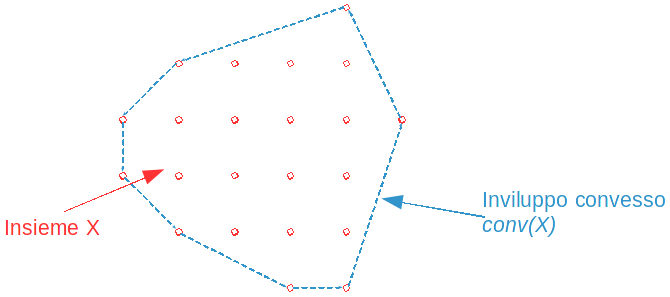
\includegraphics[height=4.5cm]{images/graph27.png}}
Si osservi che l'ottimo del problema Lagrangiano:
\begin{displaymath}
	RL_{u}
	\begin{cases}
		L(u)=Min\;cx-u(Ax-b) \\
		\;\;\;\;\;\;\;\;\;\;\;\;\;\;\;\;\;\;\;\;s.t.\;Bx\ge d \\
		\;\;\;\;\;\;\;\;\;\;\;\;\;\;\;\;\;\;\;\;\;\;\;\;\;\;x\in (0,1)
	\end{cases}
\end{displaymath}
corrisponde ad un punto estremo di $conv(X)$
\subsection{TEOREMA}
Il Lagrangiano Duale $D_{L}$ corrisponde al seguente problema di programmazione lineare.
\begin{displaymath}
D_{L}
\begin{cases}
z(D_{L})=Min\;cx \\
\;\;\;\;\;\;\;\;\;\;\;\;\;\;\;\;\;\;\;\;s.t.\;Ax\ge d \\
\;\;\;\;\;\;\;\;\;\;\;\;\;\;\;\;\;\;\;\;\;\;\;\;\;\;x\in conv(X)
\end{cases}
\end{displaymath}
dove $X=\{x:Bx\ge d,\;x\in(0,1)\}$ e $conv(X)$ è l'inviluppo convesso di $X$.
\subsubsection{Dimostrazione}
Si ricordi che:
\begin{equation*}
	D_{L}\;\;\;\;\;z(D_{L})=\underset{u\ge 0}{Max}\;[L(u)]
\end{equation*}
e, per come è stato definite $X$, il problema $RL_{u}$ diviene
\begin{equation*}
	RL_{u}\;\;\;\;\;L(u)=\underset{x\in X}{Min}\;(cx-u(Ax-b))
\end{equation*}
Quindi, il problema $D_{L}$ può essere scritto come:
\begin{equation*}
	D_{L}\;\;\;\;\;z(D_{L})=\underset{u\ge 0}{Max}\;[\underbrace{\underset{x\in X}{Min)}\;(cx-u(Ax-b))]}_{L(u)}
\end{equation*}
o anche
\begin{equation*}
D_{L}\;\;\;\;\;z(D_{L})=\underset{u\ge 0}{Max}\;[\underset{x\in conv(X)}{Min)}\;(cx-u(Ax-b))]
\end{equation*}
poichè $L(u)$ raggiunge l'ottimo in un punto estremo di $conv(X)$.\\
Indichiamo con $x^{i},\;i=1,\dots,t$ i punti estremi di $conv(X)$. Il problema $D_{L}$ può essere scritto come:
\begin{equation*}
	D_{L}\;\;\;\;\;z(D_{L})=\underset{u\ge 0}{Max}\;[\underset{1\le i\ge t}{Min}\;(cx^{i}-u(Ax^{i}-b))]
\end{equation*}
quest'ultimo problema può essere riformulato mediante la programmazione lineare come segue:
\begin{equation*}
	D_{L}
	\begin{cases}
	z(D_{L})=Max\; v \\
	\;\;\;\;\;\;\;\;\;\;\;\;\;\;\;s.t.\; v\le cx^{i}-u(Ax^{i}-b),\;i=1,\dots,t\\
	\;\;\;\;\;\;\;\;\;\;\;\;\;\;\;\;\;\;\;\;\;\textnormal{v qualsiasi} \\
	\;\;\;\;\;\;\;\;\;\;\;\;\;\;\;\;\;\;\;\;\;u\ge 0
	\end{cases}
\end{equation*}
Il duale di questo problema è il seguente
\begin{equation*}
	DD_{L}
	\begin{cases}
		z(D_{L})=Min\;\sum_{i=1}^{t}\lambda_{i}(cx^{i})\\
		\;\;\;\;\;\;\;\;\;\;\;\;\;\;\;s.t.\; \sum_{i=1}^{t}\lambda_{i}=1 \\
		\;\;\;\;\;\;\;\;\;\;\;\;\;\;\;\;\;\;\;\;\;\sum_{i=1}^{t}\lambda_{i}(Ax^{i}-b)\ge 0 \\
		\;\;\;\;\;\;\;\;\;\;\;\;\;\;\;\;\;\;\;\;\;\lambda_{i}\ge 0,\;i=1,\dots,t
	\end{cases}
\end{equation*}
Si noti che $\sum_{i=1}^{t}\lambda_{i}(cx^{i})=c(\sum_{i=1}^{t}\lambda_{i}x^{i})$ ed inoltre $\sum_{i=1}^{t}=\lambda_{i}(Ax^{i}-b)=A(\sum_{i=1}^{t}\lambda_{i}x^{i})-b(\sum_{i=1}^{t}\lambda_{i})$.\\
Quindi $DD_{L}$ può essere riscritto come
\begin{numcases}{DD_{L}}
	z(D_{L})=Min\;c(\sum_{i=1}^{t}\lambda_{i}x^{i}) \\
	\;\;\;\;\;\;\;\;\;\;\;\;\;\;s.t.\;\sum_{i=1}^{t}\lambda_{i}=1 \label{eq:3.21}\\
	\;\;\;\;\;\;\;\;\;\;\;\;\;\;\;\;\;\;\;\;A(\sum_{i=1}^{t}\lambda_{i}x^{i})\ge b(\sum_{i=1}^{t}\lambda_{i}) \label{eq:3.22}\\
	\;\;\;\;\;\;\;\;\;\;\;\;\;\;\;\;\;\;\;\;\lambda_{i}\ge 0,\;i=1,\dots,t \label{eq:3.23}
\end{numcases}
Si osservi che, per ognu t-pla $\lambda_{i},\dots,\lambda_{t}$ che soddisfa i vincoli \ref*{eq:3.21} e \ref{eq:3.23}, il punto $x=\sum_{i=1}^{t}\lambda_{i}x^{i}$ appartiene a $conv(X)$. Quindi il problema $DD_{L}$ può essere riscritto come
\begin{equation}
	DD_{L}
	\begin{cases}
		z(D_{L})=Min\;cx \\
		\;\;\;\;\;\;\;\;\;\;\;\;\;\;s.t.\;Ax\ge b \\
		\;\;\;\;\;\;\;\;\;\;\;\;\;\;\;\;\;\;\;\;x\in conv(X)
	\end{cases}
\end{equation}
$\square$

\section{Lagrangiano Duale e Rilassamento Lineare}
\subsection{TEOREMA}
\begin{equation}
	z(D_{L})\ge z(LP)
\end{equation}
\subsection{Dimostrazione}
Il rilassamento lineare $LP$ è definito come
\begin{equation}
	LP
	\begin{cases}
		z(LP)=Min\;cx \\
		\;\;\;\;\;\;\;\;\;\;\;\;\;\;\;s.t.\;Ax\ge b \\
		\;\;\;\;\;\;\;\;\;\;\;\;\;\;\;\;\;\;\;\;\;Bx\ge d \\
		\;\;\;\;\;\;\;\;\;\;\;\;\;\;\;\;\;\;\;\;\;0\le x\le 1
	\end{cases}
\end{equation}
Definiamo $\bar{X}=\{x:Bx\ge d,\;0\le x\le 1\}$, quindi
\begin{equation}
	LP
	\begin{cases}
		z(LP)=Min\;cx \\
		\;\;\;\;\;\;\;\;\;\;\;\;\;\;\;s.t.\;Ax\ge b\\
		\;\;\;\;\;\;\;\;\;\;\;\;\;\;\;\;\;\;\;\;\;x\in\bar{X}
	\end{cases}
\end{equation}
Per come abbiamo definito $\bar{X}$ è facile osservare che:
\begin{equation}
	conv(X)\subseteq\bar{X}
\end{equation}
e poichè abbiamo dimostrato che
\begin{equation}
	D_{L}
	\begin{cases}
		z(D_{L})=Min\;cx\\
		\;\;\;\;\;\;\;\;\;\;\;\;\;\;\;s.t.\;Ax\ge b \\
		\;\;\;\;\;\;\;\;\;\;\;\;\;\;\;\;\;\;\;\;\;x\in conv(X)
	\end{cases}
\end{equation}
si ha che $z(D_{L})\ge z(LP)$.\\
$\square$

\subsection{TEOREMA: $\boldsymbol{L(u)}$ è concava}
La funzione lagrangiana $L(u)$ è concava, ovvero $L(\lambda u^{1}+(1-\lambda)u^{2})\ge \lambda L(u^{1})+(1-\lambda)L(u^{2})$, $\lambda \in [0,1]$

\centerline{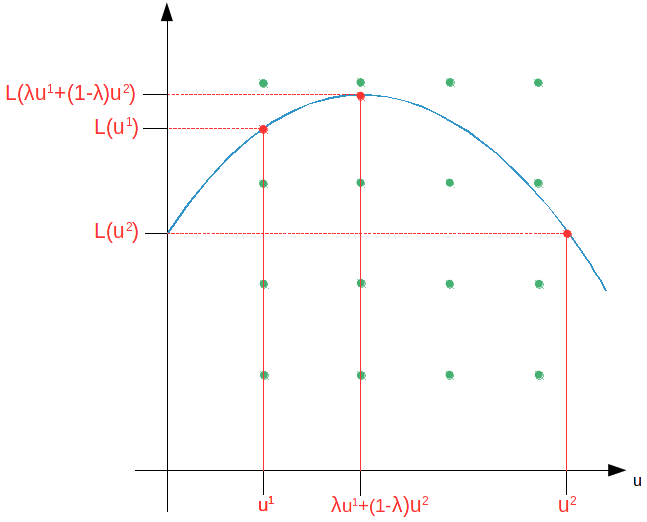
\includegraphics[height=8cm]{images/graph28.png}}

\subsubsection{Dimostrazione}
Siano $u^{1},u^{2}\ge 0$ e $u^{0}=\lambda u^{1}+(1-\lambda)u^{2}$ con $\lambda in[0,1]$.\\
Indichiamo con $x^{0}$ la soluzione ottima di $RL_{u^{0}}$:
\begin{equation}
	L(u^{0})=cx^{0}-u^{0}(Ax^{0}-b)
\end{equation}
$x^{0}$ è soluzione ammissibile di $RL_{u^{1}}$ e $RL_{u^{2}}$ quindi
\begin{flalign}
	L(u^{1})\le cx^{0}-u^{1}(Ax^{0}-b) \label{eq:3.31} \\
	L(u^{2})\ge cx^{0}-u^{2}(Ax^{0}-b) \label{eq:3.32}
\end{flalign}
Moltiplicando la \ref{eq:3.31} per $\lambda$, la \ref{eq:3.32} e sommando:
\begin{equation}
	\lambda L(u^{1})+(1-\lambda)L(u^{2})\le cx^{0}-\underbrace{(\lambda u^{1}+(1-\lambda)u^{2})}_{u^{0}}(Ax^{0}-b)=L(u^{0})
\end{equation}

\section{Subgradiente di $\boldsymbol{L(u)}$}
Un vettore è detto subgradiente di $L(u)$ in $\bar{u}$ se soddisfa
\begin{equation}
	L(u)\ge L(\bar{u})+y(u-\bar{u})
\end{equation}

\centerline{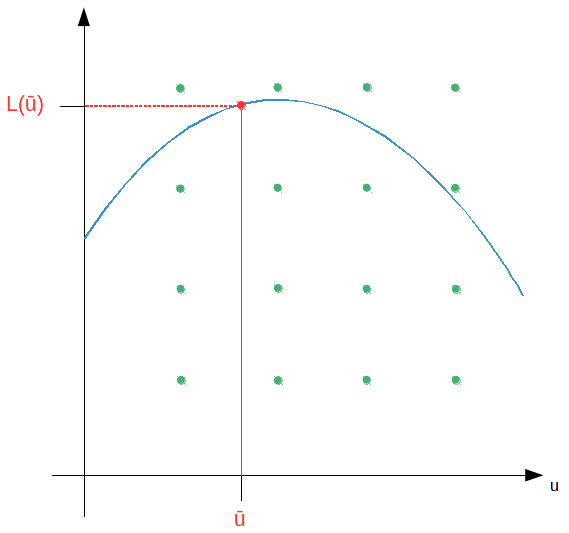
\includegraphics[height=7cm]{images/graph29.png}}

\textbf{Come calcolare $\boldsymbol{y}$?}\\
Sia $\bar{x}$ tale che
\begin{equation}
	L(\bar{u})=c\bar{x}-\bar{u}(A\bar{x}-b) \label{eq:3.35}
\end{equation}
Per ogni $u\ge 0$ si ha
\begin{equation}
	L(u)\le c\bar{x}-u(A\bar{x}-b) \label{eq:3.36}
\end{equation}
Sottraendo dalla \ref{eq:3.36} la \ref{eq:3.35} si ottiene
\begin{equation}
	L(u)=L(\bar{u})\ge -(A\bar{x}-b)(u-\bar{u})
\end{equation}
ma anche
\begin{equation}
	L(u)\le L(\bar{u})-(A\bar{x}-b)(u-\bar{u})
\end{equation}
ne segue che $y=-(A\bar{x}-b)$ è un subgradiente di $L(u)$ in $\bar{u}$

\subsection{Metodo del subgradiente}
Metodo iterativo per risolvere il lagrangiano duale
\begin{equation*}
	D_{L}
	\begin{cases}
		z(D_{L})=\underset{u\ge 0}{Max}[L(u)]
	\end{cases}
\end{equation*}
Il metodo genera una sequenza finita di punti $(u^{1},u^{2},\dots,u^{k})$ e, quindi, calcola
\begin{equation*}
	z(D_{L})=\underset{u\in \{u^{1},u^{2},\dots,u^{k}\}}{Max}[L(u)]
\end{equation*}
\subsubsection{Generazione di $\boldsymbol{u^{r}}$ in funzione di $\boldsymbol{u^{r-1}}$}
Sia $x^{r-1}$ tale che $L(u^{r-1})=cx^{r-1}-u^{r-1}(Ax^{r-1}-b)$.\\
Abbiamo dimostrato che
\begin{equation}
	L(u^{r})\le L(u^{r-1})-(Ax^{r-1}-b)(u^{r}-u^{r-1})
\end{equation}
se vogliamo che $L(u^{r})$ possa essere maggiore di $L(u^{r-1})$ è necessario che
\begin{equation}
	-(Ax^{r-1}-b)(u^{r}-u^{r-1})>0 \label{eq:3.40}
\end{equation}
Si noti che una scelta di $u^{r}$ che verifichi la suddetta condizione non è sufficiente per garantire che $L(u^{r})>L(u^{r-1})$.\\
Come definire $u^{r}$ affinchè \ref{eq:3.40} sia verificata?\\
Supponiamo che $A$ abbia $m$ righe e quindi $u=(u_{1},\dots,u_{m})$ indicando con $a^{i}\ge b_{i}$ la i-esima disequazione di $Ax\ge b$; la condizione \ref{eq:3.40} può essere scritta come
\begin{equation*}
	-\sum_{i=1}^{m}(a_{i}^{r-1}-b_{i})(u_{i}^{r}-u_{i}^{r-1})>0 \label{eq:3.40bis}
\end{equation*}
Per soddisfare \ref{eq:3.40bis} è sufficiente determinare ogni $u_{i}^{r}$ in modo che
\begin{equation}
	-(a^{i}x^{r-1}-b_{i})(u_{i}^{r}-u_{i}^{r-1})>0,\;\forall i=1,\dots,m
\end{equation}
Da cui seguono i sequenti casi:

\begin{itemize}
	\item $a^{i}x^{r-1}$: $x^{r-1}$ viola il vincolo i-esimo \\
	definisci $u_{i}^{r}>u_{i}^{r-1}$
	\item $a^{i}x^{r-1}>b_{i}$: $x^{r-1}$ soddisfa il vincolo i-esimo \\
	definisci $u_{i}^{r}<u_{r}^{r-1}$ ma imponi $u_{i}^{r}\ge 0$
	\item $a^{i}x^{r-1}=b_{i}$: $x^{r-1}$ satura il vincolo i-esimo \\
	$u_{i}^{r}$ qualsiasi (è buona norma $u_{i}^{r}=u_{i}^{r-1}$!)
\end{itemize}

\begin{enumerate}
	\item Inizializza $u^{1}=0$ e poni $r=1$ e $LB=-\infty$
	\item Risolvi:
	\begin{equation*}
		L(u^{r})
		\begin{cases}
			Min\;cx-u^{r}(Ax-b)\\
			s.t.;Bx\ge d\\
			x\in(0,1)
		\end{cases}
	\end{equation*}
	Sia $x^{r}$ la soluzione ottima\\
	Se $L(u^{r})>LB$ allora poni $LB=L(u^{r})$ e $u^{*}=u^{r}$\\
	Se $Ax^{r}\ge b$ e $u^{r}(Ax^{r}-b)=0$ allora $x^{r}$ è soluzione ottima di $P$: STOP
	\item Definisci i moltiplicatori di $u^{r+1}$
	\begin{equation*}
		u_{i}^{r+1}=Max[0,\;u_{i}^{r}-\alpha \cdot\frac{z_{UB}-L(u^{r})}{\sum_{i=1}^{m}\widetilde{y_{i}^{2}}}\cdot\widetilde{y_{i}}],\;\forall i
	\end{equation*}
	dove $\widetilde{y_{i}}=a^{i}x^{r}-b_{i}$ e $\alpha$ è una costante ($0<\alpha\le 2$).\\
	Poni $r\gets r+1$ e ritorna allo step \textit{2}.
	\item Il metodo potrebbe non arrestarsi: è quindi necessario imporre un numero massimo di iterazioni.
	\item È opportuno diminuire il valore di $\alpha$ ($\alpha\gets\alpha/2$) se per $\delta$ iterazioni consecutive $L(u)\le LB$
	\item I valori di $\alpha$ e $\delta$ vanno determinati sperimentalmente: tipicamente $\alpha=2$ e $\delta=30$.
\end{enumerate}

\subsection{Vincoli Misti}
\begin{equation*}
	z(P)
	\begin{cases}
		Min\;cx\\
		\;\;\;\;\;\;\;\;A_{1}x\ge b_{1}\;\;\;\;m_{1}\textnormal{ righe e }u^{1}\ge 0 \\
		\;\;\;\;\;\;\;\;A_{2}x=b_{2}\;\;\;\;m_{2}\textnormal{ righe e }u^{2}\in \mathbb{R}^{m_{2}} \\
		\;\;\;\;\;\;\;\;A_{3}x\le b_{3}\;\;\;\;m_{3}\textnormal{ righe e }u^{3}\le 0 \\
		\;\;\;\;\;\;\;\;Bx\ge d \\
		\;\;\;\;\;\;\;\;\;\;\;x\in\{0,1\}^{m}\;\;\;\;\;\;\;\;\;\;\;\;\;\;\;u=(u^{1},u^{2},u^{3})
	\end{cases}
\end{equation*}
\begin{equation*}
	L(u)
	\begin{cases}
		Min\;cx-u^{1}(A_{1}x-b_{1})-u^{2}(A_{2}x-b_{2})-u^{3}(A_{3}x-b_{3})\\
		\;\;\;\;\;\;\;\;s.t.\;Bx\ge d\\
		\;\;\;\;\;\;\;\;\;\;\;\;\;\;\;\;\;x\in\{0,1\}^{m}
	\end{cases}
\end{equation*}
ma anche:
\begin{equation*}
	L(u)
	\begin{cases}
		Min\;(c-u^{1}A_{1}-u^{2}A_{2}-u^{3}A_{3})x+u^{1}b_{1}+u^{2}b_{2}+u^{3}b_{3}\\
		\;\;\;\;\;\;\;\;\;\;\;\;s.t.\;Bx\ge d \\
		\;\;\;\;\;\;\;\;\;\;\;\;\;\;\;\;\;\;\;\;\;x\in\{0,1\}
	\end{cases}
\end{equation*}

\subsection{Subgradiente per vincoli mist}
Ad una generica iterazione.\\
Sia $\bar{x}$ la soluzione ottima di $L(u)$.\\
Calcola $y^{1}=A_{1}\bar{x}-b_{1}$, $y^{2}=A_{2}\bar{x}-b_{2}$, $y^{3}=A_{3}\bar{x}-b_{3}$.\\
Poni $y=(y^{1},y^{2},y^{3})$ e $t=\alpha\frac{z_{UB}-L(u)}{\displaystyle\sum_{i=1}^{m}y_{1}^{2}}$
\begin{flalign*}
	& u_{i}^{1}\gets max[0,\;u_{i}^{1}-ty_{i}^{1}],\;i=1,\dots,m_{1}\\
	& u_{i}^{2}\gets u_{i}^{2}-ty_{i}^{2},\;i=1,\dots,m_{2}\\
	& u_{i}^{3}\gets min[0,\;u_{i}^{3}-ty_{i}^{3}],\;i=1,\dots,m_{3}
\end{flalign*}

\section{Traveling Salesman Problem}
\subsection{Costi Simmetrici}
$n$ vertici, $m$ archi.\\
$G=(N,A)$: grafo non-orientato.\\
$N=\{1,\dots,n\}$ insieme dei vertici.\\
$A=\{1,\dots,m\}$ insieme degli archi. \\
\textbf{Costi simmetrici:} $c_{ij}=c_{ji}$ $\forall\;ij$
Indichiamo con $c_{l}$ il costo dell'arco $l\in A$.\\
Per ogni arco $l\in A$ siano $(\alpha_{l},\beta_{l})$ i due vertici terminali.\\
Inoltre sia $B_{i}\subset A$ l'insieme degli archi incidenti nel vertice $i\in N$.
\subsubsection{Esempio}
\begin{minipage}[l]{0.5\textwidth}
	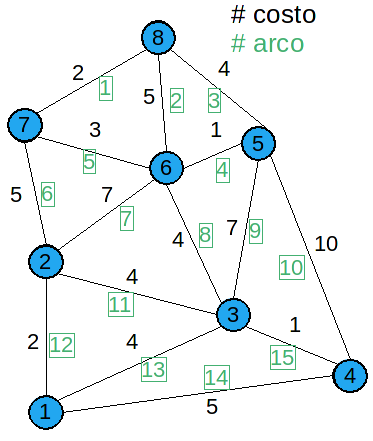
\includegraphics[height=7cm]{images/graph30.png}
\end{minipage}
\begin{minipage}[r]{0.5\textwidth}
	$n=8$ vertici\\
	$m=15$ archi\\04
	arco $14$ $\alpha_{14}=1$, $\beta_{14}=4$\\
	$B_{4}=\{10,14,15\}$\\
	$B_{3}=\{8,9,15,13,11\}$
\end{minipage}
\subsection{Fomulazione Matematica (TSP Simmetrico)}
$x_{l}=1$, se l'arco $l$ è nella soluzione ottima\\
$x_{l}=0$, altrimenti.
\begin{numcases}{}
Min\;z=\sum_{l=1}^{m}c_{l}x_{l}\\
\;\;\;\;\;\;\;\;\;\;\;\;\;\;\sum_{l\in B_{i}}x_{l}=2;\;i=1,\dots,n \label{eq:3.43}\\
\;\;\;\;\;\;\;\;\;\;\;\;\;\;\sum_{l\in K_{t}}x_{l}\ge 1;\; \forall K_{t}=(S_{t},\;N\setminus S_{t})\;\;\;\;S_{t}\subset N,\;S_{t}\neq\emptyset,\; |S_{t}|\ge 2 \label{eq:3.44}\\
\;\;\;\;\;\;\;\;\;\;\;\;\;\;x_{l}\in\{0,1\};\;l=1,\dots,m
\end{numcases}

\subsubsection{$\boldsymbol{1^{o}}$ Rilassamento Lagrangiano (SST)}
I vincoli \ref{eq:3.43} vengono portati nella fuzione obiettivo e sostituiti nella formulazione con il "surrogato" $\sum_{i=1}^{n}=(\sum_{l\in B_{i}}x_{l})=2n$.
\begin{flalign}
& L(\lambda)=min\;\sum_{l=1}^{m}c_{l}x_{l}-\sum_{i=1}^{n}\lambda_{i}(\sum_{l\in B_{i}}x_{l}-2)\\
& \sum_{l=1}^{m}x_{l}=n \label{eq:3.47} \\
& \sum_{l\in K_{t}}x_{l}\ge 1;\;\;\forall K_{t}=(S_{t},\;N\setminus S_{t})\;\;\;\;S_{t}\subset N,\;S_{t}\neq\emptyset \label{eq:3.49} \\
& x_{l}\in\{0,1\}\;\;l=1,\dots,m
\end{flalign}
\begin{flalign*}
& L(\lambda)=min\sum_{l=1}^{m}c_{l}x_{l}-\sum_{i=1}^{n}\lambda_{i}(\sum_{l\in B_{i}}x_{l}-2) \\
& L(\lambda)=min\sum_{l=1}^{m}c_{l}x_{l}+2\sum_{i=1}^{n}\lambda_{i}-\sum_{i=1}^{n}\sum_{l\in B_{i}}\lambda_{i}x_{l}
\end{flalign*}
Si noti che l'arco $l$ ha come vertici terminali $\alpha_{l}$, $\beta_{l}$ e quindi compare per $i=\alpha_{l}$ ed $i=\beta_{l}$.
\begin{flalign*}
& \sum_{i=1}^{n}\sum_{l\in B_{i}}\lambda_{i}x_{l}=\sum_{l=1}^{m}(\lambda+\lambda)x_{l} \\
& L(\lambda)=min\;\sum_{l=1}^{m}(\underbrace{c_{l}-\lambda_{\alpha_{l}}-\lambda_{\beta_{l}}}_{c'_{l}})x_{l}+2\sum_{i=1}^{n}\lambda_{i} \\
& \sum_{l=1}^{m}x_{l}=n \\
& \sum_{l\in K_{t}}x_{l}\ge 1;\;\;\;\forall K_{t}\equiv(S_{t},\;N\setminus S_{t})\;\;\;\;\;S_{t}\subset N,\;S_{t}\neq\emptyset \\
& x_{l}\in\{0,1\}
\end{flalign*}
La soluzione ottima si ottiene calcolando l'albero di costo minimo, usando i costi $(c_{l}-\lambda_{\alpha_{l}}-\lambda_{\beta_{l}})$, detto $v(SST)$ tale costo si ha che
\begin{equation}
	L(\lambda)=v(SST)+c'_{l_{min}}+2\sum_{i=1}^{n}\lambda_{i}
\end{equation}
dove $c_{l_{min}}'=min\{(c_{l}-\lambda_{\alpha_{l}}-\lambda_{\beta_{l}}):\;l\notin SST\}$

\subsection{Calcolo di $\boldsymbol{L(\lambda^{0})}$ per $\boldsymbol{\lambda^{0}=0}$}
\centerline{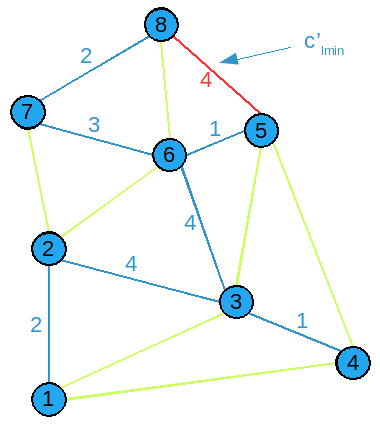
\includegraphics[height=7cm]{images/graph31.png}}
L'albero di costo minimo è $SST=\{(3,4),(6,5),(1,2),(7,8),(7,6),(2,3),(3,6)\}$ mentre l'arco minimo è $(5,8)$ e $c'_{l_{min}}=4$
\begin{equation}
	L(\lambda^{0})=v(SST)+c'_{l_{min}}=17+4=21
\end{equation}

\subsection{Calcolo Penalità Lagrangiane}
Poniamo $d_{i}=\sum_{l\in B_{i}}x_{l}$ per cui il vincolo
\begin{equation}
	\sum_{l\in B_{i}}x_{l}=2;\;\;\;\;i=1,\dots,n
\end{equation}
diviene
\begin{equation}
	d_{i}=2;\;\;\;\;i=1,\dots,n
\end{equation}
Nella soluzione prodotta per $\lambda^{0}=0$
\begin{equation}
	d^{0}=(1,2,3,1,2,3,2,2)
\end{equation}

\centerline{\boxed{
	\begin{aligned}
		& \lambda^{k}=\lambda^{k-1}-t_{k}(Ax^{k-1}-b) \\
		& \textnormal{dove} \\
		& t_{k}=\lambda_{k}\cdot\frac{(z^{*}-L(\lambda^{k-1}))}{||Ax^{k-1}-b||^{2}}
	\end{aligned}	
}}

\subsubsection{Prima iterazione: $k=1$ e $\lambda^{0}=0$, $\alpha_{1}=2$}
\begin{flalign*}
	t_{1}=2\cdot\frac{(25-21)}{\sum_{i}(d_{i}^{0}-2)^{2}}=2\cdot\frac{4}{4}=2 \\
	\lambda^{1}_{i}=0-2(d_{i}^{0}-2)\;\;\;\;i=1,\dots,n
\end{flalign*}
Quindi
\begin{flalign*}
	& \lambda_{i}^{1}>0\;\;\;\;\;\textnormal{ se }d_{i}^{0}<2 \\
	& \lambda_{i}^{1}=0\;\;\;\;\;\textnormal{ se }d_{i}^{0}=2 \\
	& \lambda_{i}^{1}<0\;\;\;\;\;\textnormal{ se }d_{i}^{0}>2 \\
	& \lambda^{1}=(+2,0,-2,+2,0,-2,0,0)
\end{flalign*}
\subsubsection{Calcolo di $\boldsymbol{L(\lambda^{1})}$}

\centerline{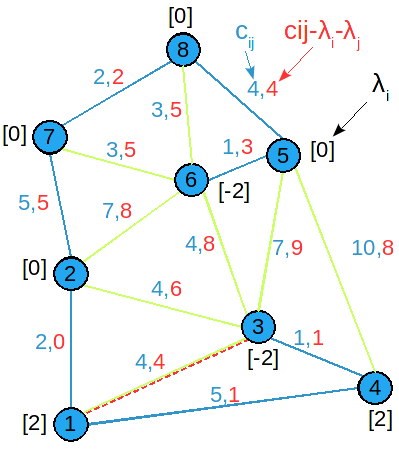
\includegraphics[height=6cm]{images/graph32.png}}
Albero di costo minimo $SST$ usando i costi $\{c_{ij},\lambda_{i}-\lambda_{j}\}$
\begin{flalign*}
	& SST={(1,2),(1,4),(3,4),(7,8),(5,6),(5,8),(2,7)} \\
	& v(SST)=16
\end{flalign*}
Nella soluzione prodotta per $\lambda^{1}=(2,0,-2,2,0,-2,0,0)$ si ha
\begin{equation*}
	d^{1}=(3,2,2,2,2,1,2,2)
\end{equation*}

\subsubsection{Nuova iterazione per $\boldsymbol{k\gets k+1}$ ossia $\boldsymbol{k=2}$}
\begin{equation*}
	\lambda_{i}^{2}=\lambda_{i}^{1}-\alpha_{2}\cdot\frac{(z^{*}-L(\lambda^{1}))}{\sum_{i}(d_{i}^{1}-2)^{2}}\cdot;\;\;\;\;i=1,\dots,n
\end{equation*}
dove $\alpha_{2}=\alpha_{1}/2=1$
\begin{equation*}
	\lambda_{i}^{2}=\lambda_{i}^{1}-1\cdot\frac{5}{2}\cdot(d_{i}^{1}-2)
\end{equation*}
Quindi
\begin{flalign*}
	& \lambda_{1}^{2}=2-\frac{5}{2}-1=-\frac{1}{2} \\
	& \lambda_{i}^{2}=\lambda_{i}^{1},\;\;\;\;i=2,3,4,5 \\
	& \lambda_{6}^{2}=-2-\frac{5}{2}\cdot(-1)=-2+\frac{5}{2}=\frac{1}{2} \\
	& \lambda_{7}^{2}=\lambda_{7}^{1},\;\lambda_{8}^{2}=\lambda_{8}^{1} \\
	& \\
	& \lambda_{2}=(-\frac{1}{2},0,-2,+2,0,\frac{1}{2},0,0)
\end{flalign*}

\subsubsection{Calcolo di $\boldsymbol{L(\lambda^{2})}$}
\centerline{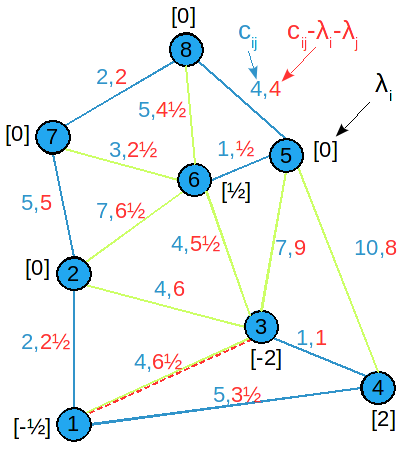
\includegraphics[height=6cm]{images/graph33.png}}
Albero a costo minimo $SST$ usando i costi $\{c_{ij}-\lambda_{i}-\lambda_{j}\}$
\begin{flalign*}
	& SST=\{(5,6),(3,4),(7,8),(1,2),(6,7),(1,4),(2,7)\} \\
	& v(SST)=17\\
\end{flalign*}
Arco a costo minimo $\notin SST$ è $(5,8)$ e $c_{l_{min}}'=4$
\begin{equation*}
	L(\lambda^{2})=v(SST)+c_{l_{min}}+2\sum_{i}\lambda_{i}=17+4+0=21
\end{equation*}
Nella soluzione per $\lambda^{2}=(-\frac{1}{2},0,-1,+2,0,\frac{1}{2},0,0)$ si ha che
\begin{equation*}
	d^{2}=(2,2,1,2,2,2,3,2)
\end{equation*}
\subsubsection{Nuova iterazione per $\boldsymbol{k=3}$, $\boldsymbol{\alpha_{3}=\frac{1}{2}\;(\alpha_{3=\alpha_{2}/2})}$}
\begin{equation*}
	\lambda_{i}^{3}=\lambda_{i}^{2}-\alpha_{3}\cdot\frac{(z^{*}-L(\lambda^{2}))}{\sum_{i}(d_{i}^{2}-2)^{2}}\cdot(d_{i}^{2}-2)
\end{equation*}
ovvero
\begin{equation*}
	\lambda_{i}^{3}=\lambda_{i}^{2}-\frac{1}{2}\cdot\frac{4}{2}\cdot(d_{i}^{2}-2)
\end{equation*}
Quindi
\begin{flalign*}
	& \lambda_{3}^{3}=-2-1\cdot(-1)=-1\\
	& \lambda_{7}^{3}=0-1\cdot 1=-1 \\
	& \textnormal{altrimenti }\lambda_{i}^{3}=\lambda_{i}^{2},\;\;\;\;\forall i\neq=3,7 \\
	& \lambda^{3}=(-\frac{1}{2},0,-1,+2,0,\frac{1}{2},-1,0)	
\end{flalign*}
\subsubsection{Calcolo di $\boldsymbol{L(\lambda^{3})}$}
\centerline{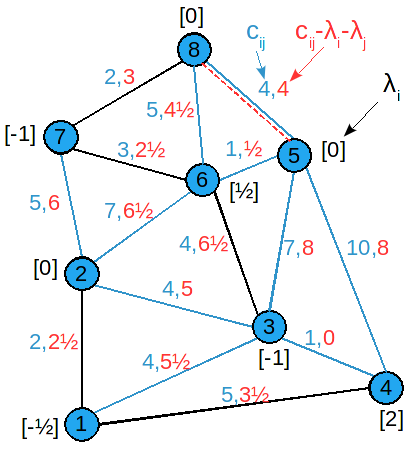
\includegraphics[height=6cm]{images/graph34.png}}
\begin{flalign*}
& SST=\{(3,4),(5,6),(1,2),(7,8),(1,4),(7,6),(3,6)\} \\
& v(SST)=17.5\\
\end{flalign*}
Arco a costo minimo $\notin SST$ è $(5,8)$ e $c_{l_{min}}'=4$
\begin{equation*}
L(\lambda^{2})=v(SST)+c_{l_{min}}+2\sum_{i}\lambda_{i}=17.5+4=21.5
\end{equation*}
\begin{equation*}
d^{3}=(2,1,2,2,2,3,2,2)
\end{equation*}
\subsubsection{Nuova iterazione per $\boldsymbol{k=4}$, $\boldsymbol{\alpha_{4}=\frac{1}{4}}$}
\begin{equation*}
	\lambda_{i}^{4}=\lambda_{i}^{3}-\frac{1}{4}\cdot\frac{3.5}{2}(d_{i}^{3}-2)
\end{equation*}
per semplificare si usi:
\begin{equation*}
	\lambda_{i}^{4}=\lambda_{i}^{3}-\frac{1}{2}\cdot(d_{i}^{3}-2)
\end{equation*}
\textit{continuare per esercizio...}

\subsection{Rilassamento 1-TREE}
\textit{Held and Karp}
\begin{itemize}
	\item Si rimuova dal grafo un vertice;
	\item Si calcolo lo shortest spanning tree (SST) sul grafo rimanente;
	\item Si aggiungano i due links di costo minimo che incidono sul vertice rimosso;
	\item Il lower bound è dato dalla somma del costo dello $SST$ e dei costi dei due link aggiunti
\end{itemize}
\centerline{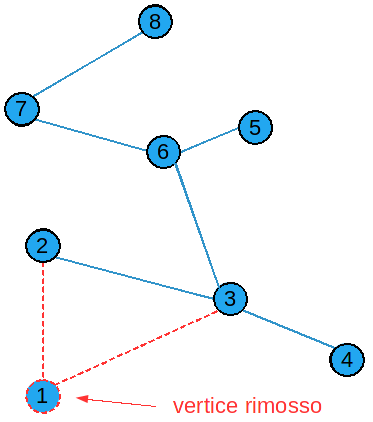
\includegraphics[height=5cm]{images/graph35.png}}
\subsection{Regola di branching TSP simmetrico}
Al nodo $K$ dell'albero decisionale: scegli un vertice $i$ il cui grado sia maggiore a $2$ è due links $a$ e $b$ che nello $SST$ incidono su $i$ e \underline{liberi}.\\
Genera $3$ nodi come segue\\
\centerline{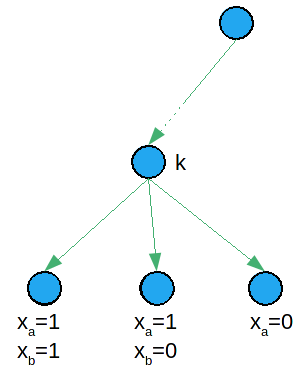
\includegraphics[height=5cm]{images/graph36.png}}